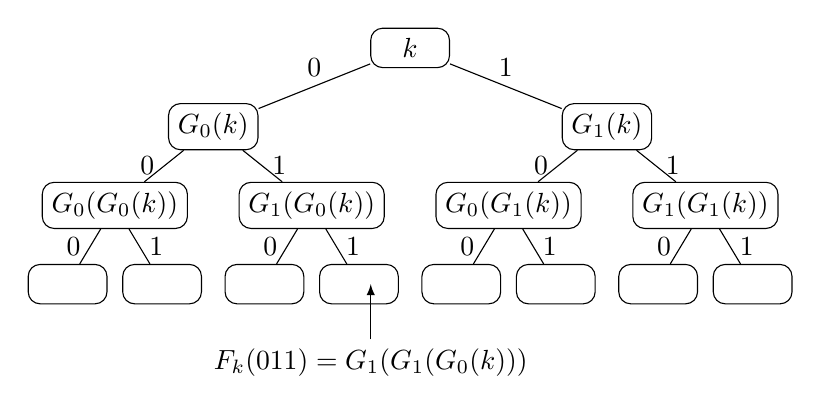
\begin{tikzpicture}[nn/.style={draw,minimum width=1cm, minimum height=0.5cm, rounded corners=1ex},level distance=1cm,
level 1/.style={sibling distance=5cm}, level 2/.style={sibling distance=2.5cm}, level 3/.style={sibling distance=1.2cm}]
%\draw[help lines] (-5,-5) grid (5,1);
\node at (0,0) [nn] {$k$}
child foreach \x in {0,1} {
  node [nn] {$G_{\x}(k)$} 
  child foreach \y in {0,1} {
    node [nn] {$G_{\y}(G_{\x}(k))$}
    child foreach \z in {0,1} {
      node [nn] {}
      \ifnum \z = 0
    edge from parent node[midway,left] {$\z$}
    \else
    edge from parent node[midway,right] {$\z$}
    \fi
    }
    \ifnum \y = 0
    edge from parent node[midway,left] {$\y$}
    \else
    edge from parent node[midway,right] {$\y$}
    \fi
  }
  \ifnum \x = 0
  edge from parent node[midway,left,above] {$\x$}
  \else
  edge from parent node[midway,right,above] {$\x$}
  \fi
};
\node (f3) at (-0.5,-4) {$F_k(011) = G_1(G_1(G_0(k)))$};
\draw[-latex] (f3) -- (-0.5,-3);
\end{tikzpicture}